\documentclass{article}

\usepackage{amsmath, mathrsfs, amssymb, stmaryrd, cancel, relsize,tikz,amsthm,comment,enumerate}

\theoremstyle{definition}
\newtheorem{Q}{Question}

\newcommand{\tvs}{\textvisiblespace}
\newcommand{\ra}{\rightarrow}
\newcommand{\la}{\leftarrow}
\newcommand{\bbN}{\mathbb{N}}

%\includecomment{comment}


\title{ITCS 532 Foundations of Computer Science\\
Week 2 - Turing Machine Variants (Homework)}
\author{Rob Egrot}
\date{}

\begin{document}
\maketitle

\begin{Q}
Let $\Sigma=\{a,b,c\}$. Let $L$ be the set of all finite strings containing the substring $ab$. Design a Turing machine that decides $L$. What regular expression describes $L$?
\end{Q}
\begin{comment}
\textbf{Solution}
\begin{center}
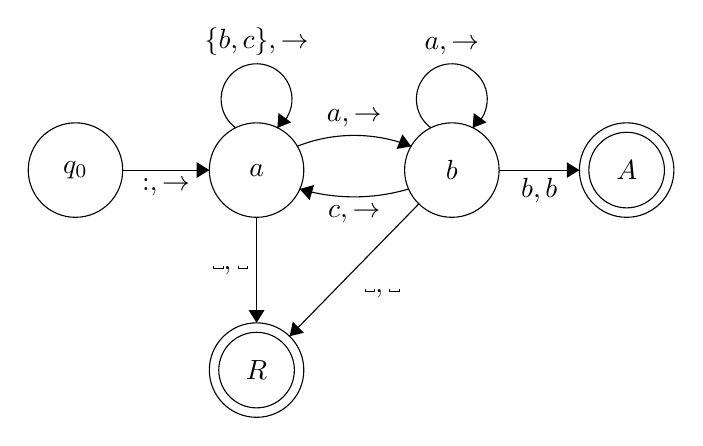
\begin{tikzpicture}[scale=0.2]
\tikzstyle{every node}+=[inner sep=0pt]
\draw [black] (15.4,-24.4) circle (3);
\draw (15.4,-24.4) node {$q_0$};
\draw [black] (26.9,-24.4) circle (3);
\draw (26.9,-24.4) node {$a$};
\draw [black] (39.3,-24.4) circle (3);
\draw (39.3,-24.4) node {$b$};
\draw [black] (50.4,-24.4) circle (3);
\draw (50.4,-24.4) node {$A$};
\draw [black] (50.4,-24.4) circle (2.4);
\draw [black] (26.9,-37.1) circle (3);
\draw (26.9,-37.1) node {$R$};
\draw [black] (26.9,-37.1) circle (2.4);
\draw [black] (18.4,-24.4) -- (23.9,-24.4);
\fill [black] (23.9,-24.4) -- (23.1,-23.9) -- (23.1,-24.9);
\draw (21.15,-24.9) node [below] {$:,\ra$};
\draw [black] (29.478,-22.889) arc (111.61948:68.38052:9.829);
\fill [black] (36.72,-22.89) -- (36.16,-22.13) -- (35.79,-23.06);
\draw (33.1,-21.7) node [above] {$a,\ra$};
\draw [black] (25.577,-21.72) arc (234:-54:2.25);
\draw (26.9,-17.15) node [above] {$\{b,c\},\ra$};
\fill [black] (28.22,-21.72) -- (29.1,-21.37) -- (28.29,-20.78);
\draw [black] (26.9,-27.4) -- (26.9,-34.1);
\fill [black] (26.9,-34.1) -- (27.4,-33.3) -- (26.4,-33.3);
\draw (26.4,-30.75) node [left] {$\tvs,\tvs$};
\draw [black] (37.2,-26.55) -- (29,-34.95);
\fill [black] (29,-34.95) -- (29.91,-34.73) -- (29.2,-34.03);
\draw (33.63,-32.22) node [right] {$\tvs,\tvs$};
\draw [black] (42.3,-24.4) -- (47.4,-24.4);
\fill [black] (47.4,-24.4) -- (46.6,-23.9) -- (46.6,-24.9);
\draw (44.85,-24.9) node [below] {$b,b$};
\draw [black] (37.977,-21.72) arc (234:-54:2.25);
\draw (39.3,-17.15) node [above] {$a,\ra$};
\fill [black] (40.62,-21.72) -- (41.5,-21.37) -- (40.69,-20.78);
\draw [black] (36.558,-25.599) arc (-73.45716:-106.54284:12.146);
\fill [black] (29.64,-25.6) -- (30.27,-26.31) -- (30.55,-25.35);
\draw (33.1,-26.6) node [below] {$c,\ra$};
\end{tikzpicture}
\end{center}

The regular expression is $\cdot ab \cdot$ if we treat the alphabet as implicit, or, if we want to specify the alphabet, we could use $(a|b|c)^\ast ab (a|b|c)^\ast$ .
\end{comment}

\begin{Q}
Let $\Sigma$ be a finite alphabet. Consider the class $\mathcal C$ of Turing machine variants over $\Sigma$ with a countably infinite number of tape heads instead of only one. So the transition function is defined by \begin{equation*}\delta:(Q\setminus H)\times \Sigma^\omega \to Q\times(\Sigma\setminus\{:\}\cup \{\la,\ra\})^\omega \end{equation*}
Let $L\subseteq \Sigma^*$ be any language over $\Sigma$. Show that there is a machine in $\mathcal C$ that decides $L$. What does this tell us about the relative power of $\mathcal C$ and the class of regular Turing machines?

HINT: To make this question easier, you can assume that the machine can tell when different tape heads are reading the same space on the tape, and that this information can be used by the transition function. If you want an extra-difficult challenge try to do without this assumption.
\end{Q}
\begin{comment}
\textbf{Solution}
With the assumption: The machine operates as follows:
\begin{enumerate}
\item Move all the tape heads to the right, so they are all reading the first symbol on the tape.
\item Move all tape heads except the first to the right, so the first is still reading the first symbol, and the rest are reading the second symbol. 
\item Move all except the first and second tape head to the right.
\item Keep following this pattern till the first blank space is found.
\item Now there are $n$ tape heads reading the $n$ characters of the input string, and the rest of the tape heads are all reading a blank space.
\item Write the transition function so that if the string being read is in $L$ the machine accepts, and it rejects otherwise.
\end{enumerate}
The assumption is used here so the machine knows which tape heads to move at each step. E.g. if heads 4 and 5 are reading the same space but heads 3 and 4 are not, it can use this information to say that head 4 must stay in place and all higher numbered heads must move right.
\newline
\newline 
This tells us this new kind of machine is much more powerful than regular Turing machines. 
\newline
\newline
Without the assumption: Let the tape heads be $h_1,h_2,\ldots$. The machine operates as follows:
\begin{itemize}
\item (Step 0) Move all the tape heads to the right, so they are all reading the first symbol on the tape.
\item (Step 1) Move all the tape heads $h_i$ such that $2|i$ to the right, and keep the others in place, except for $h_1$ which moves back to the start of the tape.
\item (Step 2) Move all the tape heads $h_i$ such that $2$ and $3$ divide $i$ to the right. Keep the others in place except $h_1$ which moves back to square 1 (as it must do this), and also move $h_3$ back to the start of the tape.
\item (Step 3) Move all the tape heads $h_i$ such that $i$ is divisible by $2,3,5$ to the right. Keep the others in place except $h_3$ which moves back to square 1, and also move $h_5$ back to the start of the tape.
\item (Step 4) Move the tape heads $h_i$ such that $i$ is divisible by $2,3,5,7$ to the right. Keep the others in place except $h_5$ which moves back to square 1, and also move $h_7$ back to the start of the tape.
\item (Step $k$) To understand the pattern here we list the prime numbers (in order) as $p_1,p_2,\ldots$. At the start of computation step $k>2$, the tape heads with numbers divisible by $p_1\times\ldots \times p_{k-1}$ are reading cell $k-1$. The head $h_{p_{k-1}}$ is also back at the start of the tape reading the $:$ symbol. The fact that $h_{p_{k-1}}$ is reading $:$ is very important, as using this we can code the machine so that it advances all tape heads with numbers divisible by $p_1\times\ldots \times p_{k}$ to the right, and also send head $h_{p_k}$ back ready for the next round.
\item At some point there will be an infinite number of tape heads reading the blank space symbol. This tells the machine the end of the input has been reached.
\item When the end has been reached, we have an infinite set of tape heads reading the first symbol of the input, another infinite set reading the 2nd symbol, and so on. Moreover, these infinite sets are distinguishable by the numbers of the heads they contain (e.g. the first contains odd numbered heads, the second contains those divisible by 2, but not by any other prime, and so on). We write the transition function so that if the string being read is in $L$ the machine accepts, and it rejects otherwise.
\end{itemize}
\end{comment}

The next questions are to revise the concept of countable and uncountable sets, because we'll need them later. You may find it useful to review the class on cardinal numbers from the 531 course.

\begin{Q}
Let $\Sigma$ be a finite alphabet. Prove that $\Sigma^*$ is countably infinite. 
\end{Q}
\begin{comment}
\textbf{Solution}
$\Sigma^*$ is the set of all finite strings using $\Sigma$, so is obviously infinite. To prove it is countable it is sufficient to find a 1-1 function $f:\Sigma^*\to \bbN$. We construct an example of a function like this. Suppose $\Sigma = \{\sigma_1,\ldots,\sigma_n\}$. Let $p_1,p_2,p_3,\ldots$ list the prime numbers in ascending order. Given a string $s = \sigma_{i_1}\sigma_{i_2}\ldots\sigma_{i_k}$, define $f(s) = p_1^{i_1}\times p_2^{i_2}\times \ldots \times p_k^{i_k}$. 

So, for example, if the alphabet is $\{ a = \sigma_0, b = \sigma_1, c=\sigma_2\}$, the string $aacb$ corresponds to $2^13^15^37^2$. I.e., the letter $a$ is at positions 1 and 2 (corresponding to $p_1 = 2$ and $p_2 = 3$, the 1st and 2nd primes), the letter $c$ is at position 3, and the letter $b$ is at position 4. 

Then $f$ is 1-1 because, by the Fundamental Theorem of Arithmetic, numbers are specified uniquely by their prime factorizations (up to reordering).
\end{comment}

\begin{Q}
Let $\Sigma$ again be a finite alphabet. Is $\wp(\Sigma^*)$ countable? Justify your answer.
\end{Q}
\begin{comment}
\textbf{Solution}
This must be uncountable so long as $\Sigma$ is non-empty, because, as proved in the notes for the 531 course, given a non-empty set $X$ we always have $|X|<|\wp(X)|$. 
\end{comment}

\begin{Q}
Recall that the union of a countable number of countable sets is countable. Let $\Sigma=\{0,1\}$ and let $X=\wp(\Sigma^*)$ be the uncountable set of all languages over $\Sigma$. Let $C_1$ and $C_2$ be countable subsets of $X$, and let $U$ be an uncountable subset of $X$. Remember that if $Y$ is a set we use $\bar{Y}$ to denote the complement of $Y$. For each of the following sets say whether it is countable, uncountable, or dependent on the choice of $C_1,C_2,U$. Justify your answers.
\begin{enumerate}[(a)]
\item$C_1\cup C_2$
\item$\bar{C_1}$
\item$\bar{U}$
\item$\bar{C_1}\cap U$
\end{enumerate} 
\end{Q}
\begin{comment}
\textbf{Solution}
\begin{enumerate}[(a)]
\item This is countable as the union of a countable number of countable sets is always countable.
\item This must be uncountable, as $C_1\cup \bar{C}_1 = X$. By part (a), if both $C_1$ and $\bar{C}_1$ were countable then $X$ would be too, but $X$ is uncountable. So, since $C_1$ is countable, $\bar{C}_1$ must be uncountable.
\item This depends on the choice of $U$. If $U = X$ then $\bar{U} = \emptyset$, which is countable. Alternatively, let $U$ be the set of all languages containing the string $s$, for some arbitrary choice of $s$. Then $U$ is in bijection with $\wp(\Sigma^*\setminus\{s\})$, which is uncountable for the same reason $\wp(\Sigma^*)$ is. This bijection takes a language $L\in U$ to $L\setminus\{s\}$, which is in $\wp(\Sigma^*\setminus\{s\})$, and conversely takes $L'\in\wp(\Sigma^*\setminus\{s\})$ to $L'\cup\{s\}$, which is in $U$. Moreover, $\bar{U} = \wp(\Sigma^*\setminus\{s\})$, and so is also uncountable.   
\item This is uncountable, for the following reason.
\begin{align*}
U &= X \cap U \\
&=(\bar{C}_1\cup C_1)\cap U \\
&= (\bar{C}_1 \cap U) \cup (C_1\cap U).
\end{align*}
Now, $(C_1\cap U)$ is countable, so $(\bar{C}_1 \cap U)$ must be uncountable as $U$ is. This last step is essentially the same argument we used in part (b).
\end{enumerate}
\end{comment}



\end{document}